\chapter{Background}\label{chapter:background}
\addcontentsline{toc}{chapter}{Background}
In questo capitolo verranno introdotti i concetti di base utili alla comprensione del contesto. Andremo ad introdurre cosa sono 
le proteine e quali sono i loro componenti principali.

\section{Amminoacidi}\label{sec:cap_sec_subsec}
% Parte presa da wikipedia https://it.wikipedia.org/wiki/Amminoacido
Gli amminoacidi sono una categoria di composti organici che hanno sia il gruppo funzionale amminico (-NH\_2), sia quello carbossilico (-COOH). La parola aminoacido 
deriva quindi proprio dall'unione dei due gruppi funzionali citati prima. Siccome sono presenti contemporaneamente un gruppo acido (carbossilico) e un gruppo basico (amminico), 
sono definite molecole anfotere. Anfotere sono sostanze chimiche che possono manifestare sia un comportamento acido che uno basico. 

\begin{figure}
    \centering
    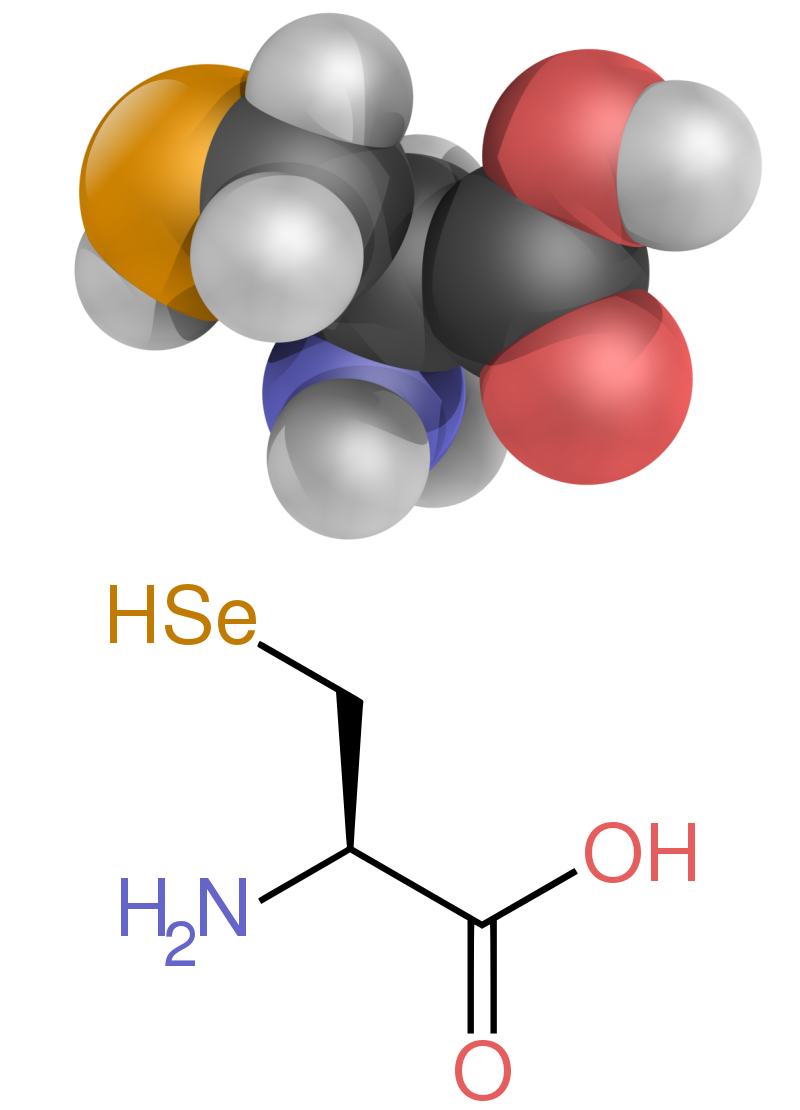
\includegraphics[width=0.3\textwidth]{Immagini/800px-Selenocysteine_skeletal_3D.png}
    \caption{Esempio di amminoacido}
    \label{fig:Amminoacido}
\end{figure}

In biochimica, ci si riferisce di solito ad un sottogruppo dei seguenti, ovvero gli $L-\alpha-amminoacidi$, ovvero amminoacidi il cui gruppo amminico e carbossilico sono 
legati allo stesso atomo di carbonio, chiamato appunto $\alpha$ e la loro configurazione è ad L, ovvero il gruppo amminico si troverà sempre alla sinistra del carbonio $\alpha$.
Sono presenti 22 $L-\alpha-amminoacidi$ che costituiscono la struttura delle proteine, anche detti amminoacidi proteinogenici. 
Oltre hai al gruppo carbosillico e al gruppo aminico, ogni amminoacido si contraddistingue dagli altri per la presenza di un residuo R, conosciuto anche con il nome di 
catena laterale.

\begin{figure}
    \centering
    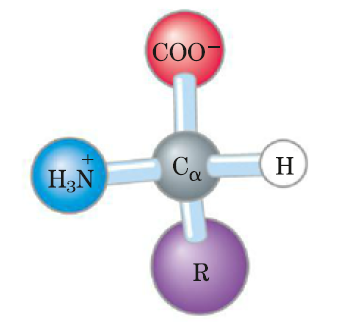
\includegraphics[width=0.4\textwidth]{Immagini/StrutturaAmminoacido.png}
    \caption{Struttura dell'amminoacido}
    \label{fig:Amminoacido}
\end{figure}
\subsection{Catena laterale}\label{subsec:es_subsec}
La catena laterale gioca degli amminoacidi gioca un ruolo importante per la determinazione delle proprietà delle proteine. Esiste una vasta diversità nelle proprietà 
chimiche delle catene laterali degli amminoacidi, tuttavia essi possono essere raggruppati in 6 classi differenti.

\begin{table}[ht]
    \centering
    \resizebox{0.99\linewidth}{!}{
        \begin{tabular}{%
            |>{\itshape}p{40mm}%
            |>{\ttfamily}p{75mm}|}
            \hline
            Tipo di catena laterale & Amminoacidi \\
            \hline
            Alifatica & Glicina, alanina, valina, leucina, isoleucina\\
            \hline
            Contenente idrossile o solfuro & Serina, cisteina, treonina, metionina\\
            \hline
            Aromatica & Fenilalanina, tiroxina, triptofano\\
            \hline
            Basica & Istidina, lisina, arginina\\
            \hline
            Acido e la sua ammide & Acido aspartico, acido glutammico, asparagina, glutammina\\
            \hline
            Ciclica & Prolina\\
            \hline
        \end{tabular}
    }
    \vspace*{2mm}
	\caption{Classi di amminoacidi}
	\label{tab:perf}    
\end{table}

La prolina non può essere inserita in una qualsiasi classe perché è ciclica. La prolina condivide la maggior parte delle proprietà 
con i gruppi alifatici. La rigidità dell'anello gioca un ruolo cruciale nella struttura delle proteine. Come già detto, 
gli amminoacidi sono i mattoni di costruzione delle proteine e la metà di questi sono anche essenziali per l'essere umano, 
poiché non è in grado di produrseli da soli.  

Gli amminoacidi in azione combinata o in azione singola sono alla base di molte attività presenti nel nostro corpo.
%%% Valuta se inserire le caratteristiche peculiari degli amminoacidi


\section{Proteine}\label{sec:cap_sec_subsec}
A livello chimico, le proteine non sono altro che macromolecole biologiche costituite da catene di amminoacidi legate insieme da un legame peptidico. Il legame 
peptidico o giunto peptidico è un legame covalente che unisce il gruppo (-NH\_2) di un amminoacido con il gruppo (-COOH) di un altro amminoacido. Negli organismi 
viventi le proteine svolgono innumerevoli funzioni, tra cui la catalisi delle reazioni metaboliche, funzione di sintesi come replicazione del DNA, la risposta a 
stimoli e il trasporto di molecole da un luogo ad un altro. Le proteine in generale si differiscono nella sequenza degli amminoacidi, che viene conservata nei geni 
e che si traduce in un particolare ripiegamento della stessa e una struttura tridimensionale specifica che caratterizza la sua attività.

A differenza di altre macromolecole biologiche come i polisaccaridi e gli acidi nucleici, le proteine sono essenziali negli organismi viventi perché prendono parte 
a praticamente tutti i processi che avvengono nelle cellule. La maggior parte appartiene alla categoria degli enzimi, che caratterizzano le reazioni biochimiche 
vitali per il metabolismo degli organismi. Hanno anche funzioni strutturali o meccaniche nei muscoli e che costituiscono il citoscheletro. Alcune sono fondamentali 
per l'invio di segnali inter ed intracellulari e nella difesa immunitaria. Una volta che sono sintetizzate all'interno del organismo, esistono per un periodo di 
tempo limitato per poi esser degradate e riciclate attraverso meccanismi cellulari. 

Le proteine possono essere purificate da altri componenti cellulari e utilizzando tecniche come: l'ultracentrifugazione; la precipitazione; l'elettroforesi; 
la cromatografia. L'avvento dell'ingengneria genetica ha portato a nuove tecniche che ne facilitano la purificazione. 

Una catena lineare di residui amminoacidi è chiamata polipeptide, ed una proteina generalmente è costituita da uno o più polipeptidi lunghi eventualmente coordinati 
a gruppi non peptidici, chiamati prostetici o cofattori. I polipeptidi che contengono meno di 20/30 amminoacidi non vengono quasi mai considerati proteine, ma più 
spesso chiamati peptidi. La sequenza degli amminoacidi in una proteina è definita della sequenza presente nel gene a sua volta codificata nel codice genetico, 
solitamente ne sono specificati 20 ma possono essere di più in alcuni organismi.

Le proteine che hanno stesso numero e tipo di amminoacidi possono differire per come vengono posti all'interno della struttura, anche una singola variazione può 
portare ad una variazione nella struttura tridimensionale della macromolecola che può rendere la proteina non funzionale. 

\subsection{Classificazione}\label{subsec:es_subsec}

Durante l'evoluzione ci sono stati duplicamenti di geni e alterazioni della funzione di una proteina che portano tutt'ora ad avere circa 500 famiglie proteiche. 
All'interno della stessa famiglia le proteine svolgono funzioni leggermente diverse, ma per quanto riguarda la loro composizione a livello di sequenza di amminoacidi
è quasi identica. Chiaramente ci sono anche casi in cui le proteine all'interno della stessa famiglia si differiscono a livello di sequenza di amminoacidi, ma hanno 
una conformazione tridimensionale molto simile. 

Si afferma quindi che nel corso dell'evoluzione si sia più conservata la conformazione tridimensionale, piuttosto che la sequenza. Si può dire che due proteine hanno 
la stessa struttura generale quando almeno un quarto della loro sequenza amminoacidi corrisponde. Si dice invece che due proteine hanno un qualche grado di parentela, 
se almeno il 30\% degli amminoacidi corrisponde. Alcune proteine possono anche essersi formate per rimescolamento dei domini proteici o per la duplicazione 
all'interno della proteina stessa con unioni accidentali di DNA. 

La classificazione può essere ottenuta grazie alla composizione chimica, alla configurazione molecolare o alla solubilità. Ci sono quindi proteine semplici che 
sono costituite da soli amminoacidi e proteine coniugate composte dalla proteina semplice e da un gruppo prostetico non proteico.

Tra le proteine semplici vi sono le proteine fibrose, tendenzialmente non solubili nei solventi acquosi e poco attaccabili dagli enzimi proteolitici, inoltre sono
presenti le proteine globulari. Mentre per quanto riguarda le proteine coniugate troviamo l'emoglobina, le clorofille e le opsine.

Si possono poi classificare le proteine in base alla funzione che compiono, ci sono le proteine strutturali che sono componenti delle strutture permanenti e che 
hanno funzione meccanica, poi trovano posto le proteine di trasporto che prendono le sostanza poco idrosolubili e ne consentono il trasporto nell'organismo e poi
trovano posto gli enzimi che sono proteine catalitiche. A queste funzioni che abbiamo brevemente descritto si aggiugono la regolazione dell'espressione dei geni, 
la duplicazione, trascrizione e traduzione del DNA, la regolazione delle reazioni metaboliche, la generazione e la ricezione degli impulsi nervosi. 

\subsection{biochimica}\label{subsec:es_subsec}

La stra grande maggioranza delle proteine sono costituite da polimeri lineari combinando 20 diversi $L-\alpha-amminoacidi$. Tutti gli aminoacidi che possono essere 
impiegati nella costruzione di proteine hanno una struttura comune, un carbonio $\alpha$ con un gruppo amminico, un gruppo carbosillico e una catena laterale 
variabile a seconda dell'aminoacido, l'unica che si distingue è la prolina che contiene un anello insolito al gruppo amminico. Le catene laterali degli amminoacidi 
hanno ognuna la loro struttura e le loro proprietà chimiche, l'effetto combinato delle catene laterali determina la struttura tridimensionale e la reattività chimica
della proteina. Una volta collegati tramite legame peptidico gli amminoacidi sono chiamati residui e la serie di carbonio, azoto e atomi d'ossigeno è nota come 
catena principale o backbone.

Il legame peptidico ha due forme di risonanza che contribuiscono al doppio legame e non permettono la rotazione attorno al suo asse, in modo tale che i carbonio 
$\alpha$ dei vari residui siano pressoche complanari. Ci sono però altri due angoli nel legame peptidico che ne determinano la forma assunta. 

\subsection{Composizione}\label{subsec:es_subsec}
Uno dei dogmi fondamentali della biologia è che ad ogni struttura tridimensionale di una proteina via sia associata una specifica funzione biochimica. In questo modo
le proteine possono essere classificate in due famiglie: le proteine globulari e le proteine a struttura estesa o fibrosa. Questa separazione riflette anche una
separazione funzionale:
\vspace{10pt}
\begin{itemize}
    \item le proteine estese o fibrose svolgono funzioni biomeccaniche quindi fornendo sostegno strutturale;
    \vspace{5pt}
    \item le proteine globulari sono coinvolte in molteplici e specifiche funzioni biologiche e sono di fondamentale importanza per l'economia cellulare.
\end{itemize}

Una proteina è formata da uno o più polipeptidi, che sono molecole con più di 10 unità di amminoacidi, eventualmente accompagnati o legati da uno o più gruppi
prostetici. Una proteina attiva può esistere solo in soluzioni salina diluita e la sua struttura dipendera esclusivamente dalle caratteristiche chimico-fisiche
della soluzione in cui è inserita, che può anche determinare modifiche strutturali e alterare le sue propieta funzionali. 

La molecola proteica risulta costituita da atomi di carbonio, ossigeno, idrogeno e azoto, può contenere anche zolfo  e, talvolta, fosforo e/o metalli.

\subsection{Struttura}\label{subsec:es_subsec}
Mettiamo un sunto sensato delle sottosottosezioni....
\subsubsection{Ripiegamento}\label{subsec:es_subsec}
Prendendo una proteina, ovvero una macromolecola formata da decina di migliaia di atomi, potrebbe assumere un numero di ripiegamenti elevati; tuttavia, non è 
cosi perché ci sono considerazioni fisiche che limitano la maggior parte dei ripiegamenti. Gli atomi non possono sovrapporsi e il loro comportamento è da immaginarsi
come delle semplici sfere, con un certo raggio detto raggio di van der Waals. Ciascun amminoacido contribuisce alla formazione della catena con tre possibili legami:
\vspace{10pt}
\begin{itemize}
    \item legame peptidico (C-N) tra il carbonio di un amminoacido e l'azoto di un amminoacido adiacente;
    \vspace{5pt}
    \item legame convezionalmente chiamato C$\alpha$-C che è presente nei due carboni della catena principale del singolo amminoacido;
    \vspace{5pt}
    \item legame C$\alpha$-N all'interno dello stesso amminoacido.
\end{itemize} 

Il legame peptidico è planare e non consente alcuna rotazione, mentre gli altri due legami possono ruotare e definiscono due angoli: l'angolo di rotazione del 
legame C$\alpha$-C è detto $\psi$; l'angolo di rotazione del legame C$\alpha$-N è $\varphi$. La conformazione degli atomi che fanno parte della catena principale 
è determinata dagli angoli descritti in precedenza. Non è pero possibile ruotare come si vuole questi angoli dato che non sono possibili collisioni steriche tra gli 
amminoacidi. Ramachandran come vedremo nella prossima sezione nel dettaglio ha individuato e rappresentato in un grafico le coppie di angoli di rotazione a seconda
delle coppie di atomi. Dal grafico si può vedere che le proteine assumono due grandi tipologie di conformazione: l'$\alpha-elica$ e il $\beta-foglietto$.

Tra gli atomi che sono all'interno di una proteina si stabiliscono dei legami che possono essere covalenti o non covalenti, i legami non covalenti sono sicuramente 
meno potenti, tuttavia il numero all'internoo di una proteina li rende fondamentali per comprendere il ripiegamento. Ci sono tre tipi di legami non covalenti:
\vspace{10pt}
\begin{itemize}
    \item il legame idrogeno, che si effettua tra un atomo di ossigeno e uno vicino ad idrogeno;
    \vspace{5pt}
    \item le attrazzioni elettrostatiche che avvengono tra gruppi laterali con cariche periferiche opposte;
    \vspace{5pt}
    \item le attrazzioni di van der Waals si verificano tra dipoli molecola istantanei indotti, tra dipoli permanenti o tra un dipolo permanente e uno corrisponde 
    indotto, nelle quali entrano in gioco forze diverse.
\end{itemize} 

Vanno aggiunte alle precendenti interazioni la tendenza dei gruppo di amminoacidi idrofobici ad avvicinarsi e unirsi tra loro, formando delle tasche idrofobiche che
sono però lontane dai legami idrogeno sempre presenti in un ambiente acquoso. Tendenzialmente questi gruppi sono posti all'interno della proteina, mentre i suoi 
amminoacidi idrofili (polari e con carica) saranno tendenzialmente all'esterno, poiché essa si trova tipicamente in un ambiente acquoso. Di solito la proteina 
tende poi ad assumere la struttura tridimensionale che ha la più bassa energia libera.

\subsubsection{Le conformazioni più comuni}\label{subsec:es_subsec}
L'$\alpha-elica$ e il $\beta-foglietto$ sono le conformazioni più comuni riscontrabili nelle catene polipeptidiche di una proteina. Una singola proteina può 
prevedere sia $\alpha-elica$ che $\beta-foglietto$ in numero variabile.

L'$\alpha-elica$ è la più comune nelle proteine, in particolare nei recettori cellulari, e si possono trovare più $\alpha-elica$ per singola proteina. L'elica è 
una delle conformazioni più favorevoli perché riduce al minimo l'energia libera. Essa si forma quando una catena polipeptidica si ripiega su se stessa con formazione
di legami idrogeno tra un legame peptidico e il quarto successivo, nel dettaglio tra il gruppo chetonico C=O dell'uno e il gruppo N-H dell'altro, e il legame 
è tra O e H. Tutti i gruppi amminici di un'elica sono rivolti verso l'N-terminale della proteina, tutti quelli chetonici verso il C-terminale, così l'elica assume 
parziale carica positiva all'N-terminale e parziale carica negativa al C-terminale.

Il $\beta-foglio$ pieghettato è la seconda conformazione più comune nelle proteine, si trova maggiormente in alcuni enzimi e nelle proteine coinvolte nella difesa 
immunitaria. Esso consiste in numerose catene polipeptidiche che si dispongono l'una adiacente all'altra, collegate in una struttura continua da brevi sequenze ad U.

\subsubsection{Livelli di organizzazione}\label{subsec:es_subsec}
All'interno della proteina si possono distinguere vari livelli di organizzazione, che possono essere tre o quattro a seconda della tipologia della stessa.
I livelli d'organizzazione sono: 
vspace{10pt}
\begin{itemize}
    \item la struttura primaria è formata dalla sequenza specifica di amminoacidi, dalla catena peptidica e il numero delle catene determina anche il ripiegamento
    della stessa;
    \vspace{5pt}
    \item la struttura secondaria consiste nella conformazione delle catene ($\alpha-elica$, $\beta-foglietto$, etc..). All'interno di una singola proteina vi può 
    essere una combinazione una combinazione di varie tipologie di sequenze;
    \vspace{5pt}
    \item il dominio è un'unità globulare o fibrosa formata da catene polipeptidiche ripiegate in più regioni compatte, costituiscono divisioni della struttura 
    terziaria, ha la caratteristica di ripiegarsi più o meno indipendentemente rispetto al resto della proteina. Molte delle proteine più complesse sono 
    aggregazioni modulari di numerosi dominii proteici;
    \vspace{5pt} 
    \item la struttura terziaria, che dal punto di vista termodinamo è quella ccon la più bassa energia libera, è rappresentata dalla configurazione tridimensionale
    completa che la catena polipeptidica assume nell'ambiente in cui si trova;
    \vspace{5pt}
    \item la struttura quaternaria deriva dall'associazione di due o più unità polipeptidiche, unite tra loro da legami deboli.
\end{itemize} 

Le proteine contenenti una parte non polipeptidica sono anche dette coniugate. Due proteine possono essere definite isoforme se a parità di struttura primaria ci sono 
differenze in uno degli altri livelli di struttura. Quando si dice denaturare una proteina significa distruggerne la sua conformazione spaziale, anche se viene 
mantenuta intatta la struttura primaria, essa non è più in grado di esplicare la sua funzione.

\subsubsection{Proteine complesse}\label{subsec:es_subsec}
Le proteine prese singolarmente sono si complesse, ma all'intermo degli organismi possono aggregarsi ad altre proteine identiche e non creando cosi dei complessi
proteici. Tutto ciò avviene grazie ai legami non covalenti che permettono ad una proteina di assumere una determinata configurazione. Nella proteina sono presenti 
una o più zone capaci di interazioni covalenti e vengono chiamate sidi di legame. Quando le proteine si uniscono insieme in un complesso proteico, le singole unità 
vengono chiamate subunità proteiche.

Ci sono complessi proteici formati da molte subunità che permettono di realizzare filamenti, poiché in un polo possiedono un sito di legame e dall'altro una struttura
proteica complementare allo stesso sito. Vi sono poi proteine la cui funzione è resa possibile proprio dalla loro struttura poco caratterizzabile e quasi casuale;
esse principalmente hanno molte funzioni all'interno della cellula. La loro caratteristica è quella di avere ridondanza di amminoacidi e bassa presenza di 
amminoacidi idrofobici. 

Ci possono essere casi in cui la proteina è esposta ad un alto livello di degradazione, esse sono quindi stabilizzate da legami di solfuro, che permettono di 
mantenere la sua conformazione.

\section{Principio di Ramachandran}\label{sec:cap_sec_subsec}
Come detto nella sezione precedente Phi $\varphi$ e Psi $\psi$ determinano la conformazione di un polipeptide. Il principio di Ramachandran ci dice quali $\alpha-elica$, 
$\beta-foglietto$ e spire sono le conformazioni più probabili da adottare per una catena polipeptidica, poiché la maggior parte delle configurazioni sono 
impossibili a causa delle collisioni steriche tra gli atomi. 

\begin{figure}
    \centering
    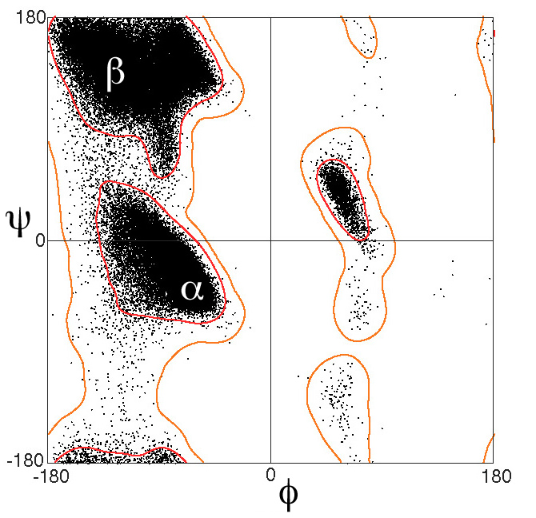
\includegraphics[width=0.4\textwidth]{Immagini/GraficoRamachandran.png}
    \caption{Esempio del grafico di Ramachandran}
    \label{fig:Amminoacido}
\end{figure}

Il principio di Ramachandran ha stabilito che solo alcune configurazioni di angoli di torsione sono stabili e presenti naturalmente nelle proteine. 
Queste configurazioni stabili sono descritte come regioni favorevoli o regioni accettabili nel grafico di Ramachandran. Le configurazioni non favorevoli o 
non accettabili sono associate con strutture instabili o anomale.

Il principio di Ramachandran viene utilizzato nella biologia strutturale per verificare la qualità delle predizioni di struttura proteica e per identificare 
eventuali errore nella modellizzazione. Viene anche utilizzato nella progettazione di proteine artificiali e nella modifica della struttura delle proteine 
esistenti per migliorare le proprietà terapeutiche o funzionali.

Non tutte le coppie di angoli teoricamente possibili sono realmente ottenibili all'interno delle strutture peptidiche in quanto impedite dalla presenza di 
ingombri sterici fra i gruppi delle catene laterali dei residui amminoacidici; le zone del grafico in cui tali contatti sterici sfavorevoli non sono presenti 
possono essere delimitate da linee di contorno, e possono essere associate ai motivi secondari assunti dalla catena. La conformazione complessiva del peptide 
è quindi definita assegnando i valori a ciascuna coppia di angoli $\psi$i, $\varphi$i per ogni amminoacido.

Nel caso della glicina, le zone di conformazioni possibili nel grafico presentano una simmetria centrale e sono molto più ampie rispetto a quelle degli 
altri amminoacidi grazie alla simmetria del residuo ed alle piccole dimensioni dell'atomo di idrogeno legato in posizione $\alpha$. Gli altri amminoacidi presentano 
invece un diagramma asimmetrico, con un insieme di zone indicanti le conformazioni ammesse meno esteso, e la cui ampiezza dipende soprattutto dalla presenza 
di gruppi stericamente ingombranti in posizione $\beta$. La presenza di catene laterali, anche lunghe, che non siano ramificate al carbonio $\beta$, come nel caso della 
leucina, ha invece una scarsa influenza e riduce solo di poco il dominio delle conformazioni permesse.

Un caso a parte si ha per la prolina, la cui struttura rigida rende possibili solo poche conformazioni in una porzione limitata del grafico.

\section{Ricerca Locale}\label{sec:cap_sec_subsec}
La ricerca locale è una tecnica euristica di ottimizzazione e risoluzione dei problemi che mira a trovare una soluzione che sia vicina alla soluzione attuale e la migliori. 
Funziona apportando piccole modifiche alla soluzione corrente e valutando i risultati, con l'obiettivo di trovare una soluzione ottimale in uno spazio di ricerca 
limitato. La ricerca locale viene spesso utilizzata nei problemi di ottimizzazione combinatoria, come il problema del commesso viaggiatore, e nell'apprendimento 
automatico, dove può essere utilizzata per ottimizzare algoritmi complessi come le reti neurali. L'idea chiave alla base della ricerca locale è evitare di rimanere 
bloccati in soluzioni non ottimali apportando una serie di piccole modifiche informate alla soluzione corrente fino a quando non viene trovata una soluzione ottimale.

La ricerca locale è un sottocampo di:
\vspace{10pt}
\begin{itemize}
    \item Metaheuristic: è una procedura o euristica di livello superiore progettata per trovare, generare o selezionare un'euristica che può fornire una soluzione
    sufficientemente buona a un problema di ottimizzazione, in particolari con informazioni incomplete o limitate capacità di calcolo;
    \vspace{5pt}
    \item Stochastic optimization: sono metodi di ottimizzazione che generano e utilizzano variabili casuali; I metodi di ottimizzazione stocastica generalizzano metodi 
    deterministici per problemi deterministici;
    \vspace{5pt}
    \item Mathematical optimization: è la selezione di un elemento migliore rispetto ad un qualche criterio, da un insieme di alternative disponibili; Nell'approccio 
    più generale, un problema di ottimizzazione consiste nel massimizzare o minimizzare una funzione reale scegliendo sistematicamente i valori di input 
    all'interno di un insieme consentito e calcolando il valore della funzione.
\end{itemize}

La maggior parte dei problemi può essere formulata in termini di spazio di ricerca e target in diversi modi. Ad esempio, per il problema del commesso viaggiatore una 
soluzione può essere un percorso che tocca tutte le città e l'obiettivo è trovare il percorso più breve. Ma una soluzione può anche essere un percorso, che può anche 
contenere un ciclo.

Un algoritmo di ricerca locale parte da una soluzione candidata e quindi si sposta iterativamente verso una soluzione vicina; un quartiere è l'insieme di tutte le 
possibili soluzioni che differiscono dalla soluzione attuale per la minima misura possibile. Ciò richiede la definizione di una relazione di vicinato nello spazio 
di ricerca. Ad esempio, l'intorno della copertura del vertice è un'altra copertura del vertice che differisce solo per un nodo. Per la soddisfacibilità booleana, 
i vicini di un'assegnazione booleana sono quelli che hanno una singola variabile in uno stato opposto. Lo stesso problema può avere più quartieri distinti definiti 
su di esso; l'ottimizzazione locale con quartieri che implicano la modifica di fino a k componenti della soluzione viene spesso definita k-opt.

Tipicamente, ogni soluzione candidata ha più di una soluzione vicina; la scelta di quale selezionare viene presa utilizzando solo le informazioni sulle soluzioni 
nelle vicinanze dell'assegnazione corrente, da cui il nome ricerca locale. Quando la scelta della soluzione del vicino è fatta prendendo quella che massimizza 
localmente il criterio, cioè: una ricerca avida, la metaeuristica prende il nome di hill climbing. Quando non sono presenti vicini in miglioramento, 
la ricerca locale è bloccata in un punto localmente ottimale. Questo problema di ottimo locale può essere risolto utilizzando i riavvii (ricerca locale ripetuta 
con diverse condizioni iniziali), la randomizzazione o schemi più complessi basati su iterazioni, come la ricerca locale iterata, sulla memoria, come 
l'ottimizzazione della ricerca reattiva, su modifiche stocastiche senza memoria, come la simulated annealing.

La ricerca locale non fornisce una garanzia che una determinata soluzione sia ottimale. La ricerca può terminare dopo un determinato periodo di tempo o quando la 
migliore soluzione trovata fino a quel momento non è migliorata in un determinato numero di passaggi. La ricerca locale è un algoritmo anytime: può restituire 
una soluzione valida anche se viene interrotta in qualsiasi momento dopo aver trovato la prima soluzione valida. La ricerca locale è in genere un'approssimazione 
o un algoritmo incompleto, poiché la ricerca potrebbe interrompersi anche se la migliore soluzione corrente trovata non è ottimale. Ciò può accadere anche se 
la terminazione avviene perché la migliore soluzione attuale non può essere migliorata, poiché la soluzione ottima può trovarsi lontano dall'intorno delle 
soluzioni attraversate dall'algoritmo.

Schuurman \& Southey propongono tre misure di efficacia per la ricerca locale (profondità, mobilità e copertura):
\vspace{10pt}
\begin{itemize}
    \item Profondità: il costo dell'attuale (migliore) soluzione;
    \vspace{5pt}
    \item Mobilità: la capacità di spostarsi rapidamente in diverse aree dello spazio di ricerca (mantenendo bassi i costi);
    \vspace{5pt}
    \item Copertura: quanto sistematicamente la ricerca copre lo spazio di ricerca, la distanza massima tra qualsiasi incarico inesplorato e tutti gli incarichi
    visitati.
\end{itemize}

Ipotizzano che gli algoritmi di ricerca locale funzionino bene, non perché abbiano una certa comprensione dello spazio di ricerca, ma perché si spostano 
rapidamente in regioni promettenti ed esplorano lo spazio di ricerca a basse profondità nel modo più rapido, ampio e sistematico possibile.

\subsection{Tipologie di ricerca locale}\label{subsec:es_subsec}
La ricerca locale si basa sul presupposto che il miglioramento di una soluzione che si trovi nelle immediate vicinanze di quest'ultima (vicinato).
Data una qualsiasi soluzione euristica (nodo corrente) la ricerca locale verifica l'esistenza di soluzioni migliori nell'insieme delle soluzioni più vicine 
(nodi vicini). Ad esempio, un algoritmo di ricerca locale può essere utilizzato per risolvere il problema del commesso viaggiatore. 
Le tecniche di ricerca locale consentono di raggiungere risultati sia nella ricerca delle soluzioni a un problema (problem solving) e sia 
nell'ottimizzazione. Appartengono alla categoria degli algoritmi di ricerca locale i seguenti algoritmi:
\begin{itemize}
    \item Ricerca hill climbing: L'algoritmo di ricerca hill climbing è una tecnica di ricerca locale in cui il nodo corrente è sostituito con il nodo migliore;
    \vspace{5pt}
    \item Simulated annealing: L'algoritmo di Simulated annealing o Annealing simulato (SA) è un algoritmo probabilistico-metaeuristico di ottimizzazione 
    della ricerca in uno spazio di ricerca di grandi dimensioni. Il suo nome prende spunto dal processo metallurgico che consente di riaggregare la materia fusa 
    dei metalli in base a determinate caratteristiche comuni. Nell'algoritmo di simulated annealing un processo di selezione consente l'eventuale sostituzione 
    della soluzione del nodo corrente con quella di un nodo selezionato casualmente da una lista di soluzioni candidate;
    \vspace{5pt}
    \item Beam Search. La beam search è una ricerca locale basata su tecniche euristiche. La beam search ( ricerca di fascio ) esplora un fascio limitato di 
    nodi promettenti (soluzioni parziali) dello spazio di ricerca e li analizza con una ricerca locale. Utilizzando le tecniche euristiche l'algoritmo beam search 
    consente di riconoscere quando una soluzione parziale è anche una soluzione completa.
\end{itemize}



\subsection{Euristiche}\label{subsec:es_subsec}
Un algoritmo di tipo Ricerca Locale appartengono alla classe delle euristiche di miglioramento. Sono euristici quegli algoritmi che non garantiscono di fornire 
la soluzione ottima. Ovvero, data una soluzione iniziale ammissibile s, essa è migliorata attraverso successive trasformazioni di s.

Le euristiche sono quindi strategie che aiutano a trovare una soluzione ottimale in una ricerca locale. Ecco alcune delle eurisiche più comuni utilizzate nella 
ricerca locale:
\vspace{10pt}
\begin{itemize}
    \item First-Improvement: Questa euristica cerca sempre la prima soluzione migliore rispetto alla soluzione corrente. Il vantaggio di questa euristica è 
    che è molto veloce, poiché interrompe la ricerca non appena viene trovata una soluzione migliore. Tuttavia, il suo limite è che potrebbe non essere in 
    grado di trovare la soluzione ottimale, poiché potrebbe fermarsi presto;
    \vspace{5pt}
    \item Best-Improvement: Questa euristica cerca sempre la migliore soluzione possibile rispetto alla soluzione corrente. Il vantaggio di questa euristica 
    è che è molto precisa, poiché cerca sempre la soluzione migliore. Tuttavia, il suo limite è che potrebbe essere molto lenta, poiché deve valutare 
    tutte le soluzioni possibili prima di scegliere la migliore;
    \vspace{5pt}
    \item Stochastic Hill Climbing: Questa euristica cerca una soluzione migliore casualmente. Il vantaggio di questa euristica è che è molto flessibile, 
    poiché cerca soluzioni in modo casuale. Tuttavia, il suo limite è che potrebbe essere impreciso, poiché potrebbe scegliere soluzioni subottimali;
    \vspace{5pt}
    \item Simulated Annealing: Questa euristica cerca una soluzione migliore basata sulla probabilità. Il vantaggio di questa euristica è che è molto 
    precisa, poiché cerca soluzioni basate sulla probabilità. Tuttavia, il suo limite è che potrebbe essere molto lenta, poiché deve valutare molte 
    soluzioni prima di scegliere la soluzione migliore;
    \vspace{5pt}
    \item Variable Neighborhood Search: Questa euristica cerca soluzioni migliori cambiando continuamente il vicinato della soluzione corrente. Il vantaggio 
    di questa euristica è che è molto flessibile, poiché cerca soluzioni in molti vicinati diversi. Tuttavia, il suo limite è che potrebbe essere molto lenta, 
    poiché deve valutare molte soluzioni prima di scegliere la soluzione migliore;
    \vspace{5pt}
    \item Greedy Algorithm: Questa euristica seleziona sempre la soluzione che sembra essere la migliore in un determinato momento. Il vantaggio di questa 
    euristica è che è molto veloce, poiché seleziona sempre la soluzione migliore. Tuttavia, il suo limite è che potrebbe non essere in grado di trovare la 
    soluzione ottimale, poiché seleziona sempre la soluzione migliore in un dato momento, senza preoccuparsi delle conseguenze future. Pertanto, 
    è importante utilizzare questo algoritmo con cautela e verificare che la soluzione ottenuta soddisfi i requisiti del problema.
\end{itemize}

\section{Hydropathic INTeractions HINT}\label{sec:cap_sec_subsec}
% File preso da Federica Agosta https://link.springer.com/article/10.1007/s10822-022-00477-y
%https://it.wikipedia.org/wiki/Forza_intramolecolare
La valutazione della stabilità intramolecolare di una proteina gioca un ruolo fondamentale nella comprensione del loro comportamento e nel meccanismo di azione. Piccole alterazioni strutturali possono impattare l'attività biologica e di conseguenza la modulazione farmacologica. 
L'analisi della struttura tridimensionale della proteina e la risultante stabilità permettono di predirre un possibile meccanismo di attivazione e rivelano nuove strategie per scoprire nuovi farmaci. Ogni modifica apportata alla struttura di una proteina porta quasi sicuramente ad una variazione del suo meccanismo di azione, e valutare la stabilità di una proteina mutata può essere molto costoso in termini di tempo.
La stabilità delle proteine mutate è influenzata dall'interazione intramolecolare, ovvero sono forze che permettono di creare e tenere insieme una struttura. Nel tentativo di analizzare la stabilità proteica, sono stati sviluppati molti metodi che svariano in diversi approcci dai meccanismi molecolari basati su force field fino a tecniche di machine learning. Tuttavia, questa pratica risulta essere molto costosa, specialmente quando sono presenti un elevato numero di mutazioni. Uno degli aspetti fondamentali su cui è basato HINT è dovuta al fatto che la stabilità delle proteine mutate è dimostrato essere influenzata dalle interazioni intramolecolari. Le strutture native delle proteine sono relativamente stabili poiché si formano come risultato di un equilibrio tra le varie forze non covalenti a cui sono soggette: i legami idrogeno, i legami ionici, le forze di Wan der Walls e le interazioni idrofobiche. In generale le interazioni chimiche deboli sono attrazzioni tra atomi appartenenti o alla stessa molecola (intramolecolari) o a molecole diverse (intermolecolari). A differenza dei legami covalenti che legano gli atomi tra loro, le interazioni chimiche deboli non sono forti abbastanza per legare tra loro atomi isolati. Per questo le interazioni chimiche deboli si formano e si rompono in continuazione alla temperatura fisiologica dell'organismo. a meno che, cumulandosi in gran numero, esse non diano collettivamente stabilità alle strutture che contribuiscono a generare.

HINT è stato sviluppato sulla base dei lavoro svolto da (indica il personaggio) che ha esteso il metodo fragment per la predizione dei $\log P\_o/v$ (coefficiente di partizione per il trasferimento di soluti in 1-ottanolo/acqua), cio permette di quantificare le interazioni idrofobiche e polari tra o all'interno dei molecole. La funzione di energia intramolecolare di HINT può essere calcolata rapidamente dalla struttura in termini di somma di punteggi d'interazione atomo-atomo. Il punteggio intramolecolare viene calcolato come somma delle interazioni idrofobiche e polari tra tutte le coppie di atomi considerando l'area accessibile al solvente. Le interazioni idrofobiche si verificano quando le molecole non polari si avvicinano tra di loro in un solvente polare, come l'acqua. Le molecole non polari tendono a respingersi reciprocamente e ad attirarsi con le molecole del solvente. Il processo anche noto come esclusione dei solventi, porta alla formazioni di molecole non polari all'interno del solvente. Le molecole non polari quindi cercano di organizzarsi in modo tale da minimizzare il contatto con il solvente e massimizzare le interazioni tra di loro. 

Il punteggio energetico di HINT intramolecolare consente quindi di calcolare tutte le interazioni idropatiche (idrofobiche e polari) che si verificano nella molecola e ne consentono di valutare la stabilità termodinamica. Dato il suo livello di sensibilità nell'individuare piccole differenze di energie verrà poi utilizzato per stimare la stabilità della Glicoproteina spike del SARS-CoV-2.

\section{Shortest Path}\label{sec:cap_sec_subsec}
Lo shortest path è un importante concetto nell'ambito dell'informatica cosi come nell'ingegneria e nella matematica applicata. Essa si riferisce al percorso più
breve tra due punti in un grafo, ovvero insieme di nodi collegati da archi. 

Esso è molto importante per esempio nel campo della robotica, viene utilizzato per pianificare il percorso del robot, consentendogli di evitare ostacoli e
raggiungere il suo obiettivo in modo efficiente. Possiamo trovare lo stesso concetto applicato nelle reti di telecomunicazioni, poiché viene utilizzato per instradare
il traffico tra due nodi garantendo una comunicazione efficiente e affidabile. Viene anche usato in algoritmi di routing per cercare di minimizzare il tempo di ritardo.
Chiaramente esso si adatta bene nel campo della logistica dove è necessario ottimizzare il trasporto delle merci o delle persone. Infine, trova applicazione anche nel
campo della progettazione di circuiti elettronici.

\subsection{Algoritmo A*}\label{subsec:es_subsec}
L'algoritmo A* è spesso utilizzato nella risoluzione del problema dello shortest path, ovvero per trovare il percorso più breve tra due nodi in un grafo pesato. 
L'algoritmo A* utilizza una funzione di stima euristica per guidare la ricerca verso il percorso più breve, permettendo di ottenere un'efficace combinazione di completezza e velocità nell'individuare la soluzione.

Nella versione dello shortest path risolto con l'algoritmo A*, ogni nodo del grafo viene valutato in base alla sua distanza dal nodo di partenza, la stima della distanza dal nodo di arrivo e il costo totale del percorso, ovvero la somma della distanza dal nodo di partenza e della stima della distanza dal nodo di arrivo. In questo modo, l'algoritmo A* tiene traccia del percorso più breve scoperto fino a quel momento e lo utilizza per determinare quale nodo espandere successivamente.

L'algoritmo A* può essere ulteriormente ottimizzato attraverso l'utilizzo di tecniche come la memorizzazione della distanza minima calcolata per ogni nodo, in modo da ridurre il numero di espansioni necessarie. Inoltre, l'algoritmo A* può essere utilizzato con successo in grafi di grandi dimensioni, grazie alla sua capacità di selezionare le espansioni più promettenti e di escludere le aree meno promettenti del grafo.

\subsection{Esempio}\label{subsec:es_subsec}
In questo esempio, la funzione A\_star prende in input la cella di partenza 'start', la cella di arrivo 'goal' e una rappresentazione del labirinto come 'graph'. La funzione A\_star esplora le celle adiacenti alla cella corrente, calcola il costo del percorso per ogni cella e aggiunge le celle alla coda di priorità. La coda di priorità è ordinata in base al costo totale, che è la somma del costo del percorso e della stima euristica. La funzione A\_star restituisce il percorso più breve dal punto di partenza al punto di arrivo.

\begin{minipage}{\textwidth}
	\begin{lstlisting}[caption={Algoritmo A*}]
		# Definizione della funzione di costo
		def cost(current, next):
			if current[0] == next[0] or current[1] == next[1]:
				return 1
			else:
				return math.sqrt(2)
		
		# Definizione della funzione euristica
		def heuristic(current, goal):
			return math.sqrt((current[0]-goal[0])**2 + (current[1]-goal[1])**2)
		
		# Definizione dell'algoritmo A*
		def A_star(start, goal, graph):
			queue = []
			heapq.heappush(queue, (0, start, []))
			visited = set()
			
			while queue:
				_, current, path = heapq.heappop(queue)
				if current == goal:
				return path + [current]
				if current in visited:
					continue
				visited.add(current)
				for neighbor in graph[current]:
					if neighbor in visited:
						continue
					new_cost = cost(current, neighbor)
					total_cost = new_cost + heuristic(neighbor, goal)
					heapq.heappush(queue, (total_cost, neighbor, path + [current]))
			return None
	\end{lstlisting}
\end{minipage}

